Organizations have their own business goals and they need software systems to satisfy those goals, sometimes with crosscutting stakeholders concerns. One of the key challenges to building systems that meet the goals of large numbers of stakeholders is integrating and reusing existing systems, while adding new functionality to support the business processes and to respond to changes in the business. Software Architecture is a bridge between those goals and the final resulting system. Software Architecture comprehends the set of structures needed to reason about the system, which comprise software elements, relations among them, and properties of both. In the ending of the 20th century, new approaches to system architecture have emerged which aim to structure a complex system around units of capability, called services \cite{bass2007software,Demchak2007,krogdahl2005service}.

This is the context in which \acrfull{SOA} is placed, that has emerged as a widely accepted solution to this challenge allowing a homogeneous enterprise-wide solution satisfying objectives that include an easy and flexible integration with legacy systems and simplifying business processes. Software architecture can be composed by several design patterns simultaneously to obtain its aim and \acrshort{SOA} is a paradigm, a design pattern, not a complete architecture. This design pattern was already used since the beginning of 1990s, mainly in \acrfull{SOAP} \cite{erl2008soa,ZurMuehlen2005} form. In the middle of 2000 years, the \acrfull{REST} \cite{Severance2015,ZurMuehlen2005} form began to spread and today its hardy do say witch proportion news applications are made in one or other form, existing intermediary forms, between both \cite{ZurMuehlen2005}. \acrshort{SOA} is a sort of architecture that use standards-based infrastructure to forge large-scale systems out of loosely coupled, inter-operable services, distributed, invocable, publishable and business oriented that can act like providers, consumers or \acrfull{IT} elements that join providers and consumers. \acrshort{SOA} can create systems-of-systems by mapping existing systems into services, then orchestrating communication between the services. New functionality can be created by either adding new services or modifying communication among existing services with low costs, innovators services to clients, agile adaption, and reaction to opportunity and weakness competitiveness \cite{bass2007software,Demchak2007,Shi2000,idoughi2010towards,Meijer2011,Chehili2013,Bianco2007,Jamek2015}.

\acrshort{SOA} also can be understood like an architectural style and uses services as building blocks to embrace changes in the business environment by composing of services and creating composite services already existing with applications in a technology heterogeneous environment \cite{Shahrbanoo2012,Sloane2008a}. The business and technical processes are implemented as services and each service represents a particular functionality that maps explicitly to a step in a business process \cite{Arsanjani2006a2006}. In this way, service can be understood as any task or function provided by an organization, aligned to business, well defined and isolated from other tasks (autonomy principle) \cite{erl2008soa} and Service orientation help organizations consistently deliver sustainable business value, with increased agility and cost effectiveness, in line with changing business needs \cite{arsanjani2009soa}. In general, the basic Service Consumer software is simply a browser or browser-like ``thin client'', with little or no application software stored locally \cite{Sloane2008a}.

In \citet{erl2008soa} it is possible to see eight principles that a service-oriented solution should follow: 
\begin{enumerate}
\item Standardized Service Contract: a service should express its purpose and capacities through a contract;
\item Service Loose Coupling: the dependencies among the service’s contract, implementation and consumers should be minimal;
\item Service Abstraction: a service should hide its implementation details to keep its consumers loosely coupled;
\item Service Reusability: services should be corporate resources, agnostic to functional contexts;
\item Service Autonomy: a service should have control over its environment and resources, while remaining isolated from other services;
\item Service Statelessness: services should only hold state information when necessary in order to not compromise its availability or scalability; 
\item Service Discoverability: services should be easily discovered and understood to foster reuse;
\item Service Composability: it should be possible to create services from the composition of other services in order to produce sophisticated solutions according to business needs requirements and fostering reuse of existing assets 
\end{enumerate}

As it is possible to see in figure \ref{fig:estilo-SOA}, \acrshort{SOA} is not just a set of services connected together. The services consumers and the services providers are connected through an infrastructure responsible to implementing many of the principles of \acrshort{SOA}, such as discoverability and composability, as well as responsible for transforming data according to standardized service contracts and dealing with security issues.

\begin{figure}[ht]
\centering
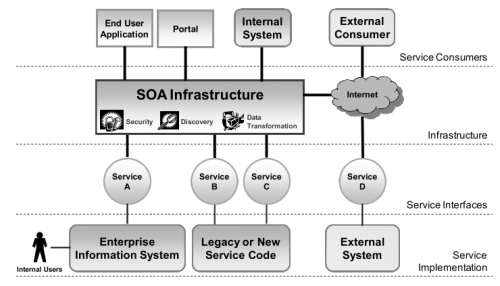
\includegraphics[width=0.8\linewidth]{images/SOA_GRAY.png}
\caption{SOA overview}
\label{fig:estilo-SOA}
\end{figure}
